% Shared preamble for the English summaries in this repository.
\documentclass[11pt,a4paper]{article}
\usepackage[margin=2.2cm]{geometry}
\usepackage[T1]{fontenc}
\usepackage[utf8]{inputenc}
\usepackage{lmodern}
\usepackage{amsmath,amssymb}
\usepackage{graphicx}
\usepackage{booktabs}
\usepackage{enumitem}
\usepackage[hidelinks]{hyperref}
\setlist{itemsep=2pt,topsep=4pt}
\setlength{\parindent}{0pt}
\setlength{\parskip}{5pt}
\graphicspath{{figures/}}
\newcommand{\summaryheader}[3]{%
  \begin{center}
    {\Large\bfseries #2}\\[3pt]
    {\large #1}\\[3pt]
    {\small Arshia Goshtasbi \textbullet{} MSc Electrical Engineering (Control), Iran University of Science and Technology \textbullet{} #3}
  \end{center}
  \vspace{2pt}\hrule\vspace{8pt}\par}

\begin{document}
\summaryheader{Machine Learning, Homework 3}{KNN and Bagging, Naive Bayes, Perceptron and Bayes' Rule}{Spring 1404 (2025)}

\textbf{Notebook} (\texttt{employee\_attrition.ipynb}). The data are 902 employees from the IBM HR Analytics attrition set (35 columns). I explored income against years at the company and by department: R\&D has the lowest average monthly income (6074) and Sales the highest (6817). I then label-encoded the categorical columns, dropped the three constant columns, made a 70/30 split and standardised the features. I wrote a KNN classifier from scratch and swept $K\in\{1,3,\dots,15\}$. The best was $K=9$ with test accuracy $0.830$. Its recall on the minority class (left the company) is only $0.20$, because 216 of the 271 test employees stayed. Bagging 9-NN models gave accuracy $0.827$ with the same weakness (Figure~\ref{fig:cm}).

\begin{figure}[h]\centering
  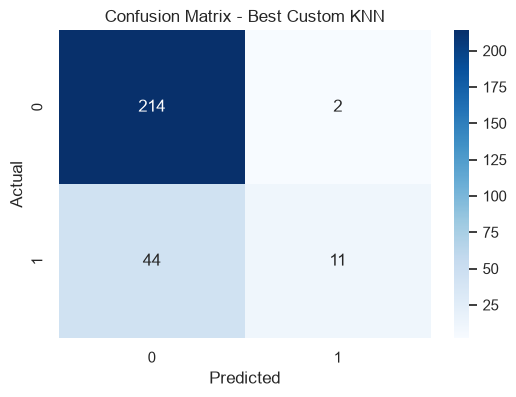
\includegraphics[width=.40\linewidth]{employee_attrition_cell17_1.png}\hspace{1em}
  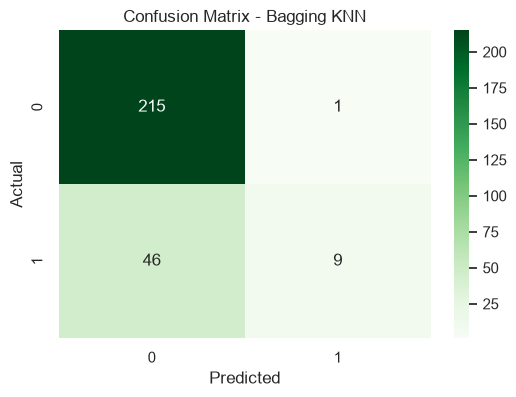
\includegraphics[width=.40\linewidth]{employee_attrition_cell23_1.png}
  \caption{Confusion matrices of the from-scratch 9-NN (left) and bagged KNN (right).}\label{fig:cm}
\end{figure}

\textbf{Written part.}
\begin{description}
  \item[Naive Bayes with zero counts.] I built four training examples where $P(A{=}1\mid C{=}0)=0$ and $P(B{=}1\mid C{=}1)=0$. A test case with $A=B=1$ then has zero likelihood under both classes, so normalising the posterior divides by zero. That observation is inconsistent with the model; Laplace smoothing avoids it.
  \item[Perceptron by hand.] From $w=(0,0)$, $b=0$, $\eta=1$, only the first sample $(1,2)$ triggers an update. This gives $w=(1,2)$ and $b=1$, after which all four points are classified correctly. The data are linearly separable (for example by $x_1+x_2=0$), so the second epoch makes no update. I also explained why the perceptron never settles when the data are not linearly separable.
  \item[Rare-disease test.] With prevalence $0.5\%$, sensitivity $90\%$ and specificity $95\%$: $P(\text{disease}\mid +)=\frac{0.9\cdot0.005}{0.9\cdot0.005+0.05\cdot0.995}\approx8.3\%$. With perfect sensitivity this only rises to $\approx9.1\%$, because false positives from the large healthy population dominate. The test alone is not enough; symptoms, history and a confirmatory test are needed.
\end{description}
\end{document}
